\documentclass[10pt,a4paper,twocolumn]{article}
\RequirePackage[italian]{babel}
\usepackage[utf8]{inputenc}
\usepackage{amsmath}
\usepackage{amsfonts}
\usepackage{amssymb}
\usepackage{graphicx}

\author{M. Faretra, G. Marini, A. Martinelli}
\title{\textbf{Raccolta accurata di fatti da testo in linguaggio naturale di Wikipedia}\\Ricreare Lector utilizzando DBpedia}
\begin{document}
	
\maketitle
		
\section*{RIASSUNTO}
		
Molti approcci sono stati tentati nell'ultimo periodo per estrarre informazione da Wikipedia sotto forma di fatti (entità, relazione, entità) per il popolamento di Knowledge Graphs, in particolare sfruttando le informazione contenute nelle sue \textit{infoboxes}. Tuttavia queste strutture dati riportano solo una piccola parte delle informazioni contenute negli articoli. Infatti nel testo libero si concentra la maggior parte dei fatti estraibili, la rilevazione di essi però risulta più problematica, trovandosi all'interno di un testo in linguaggio naturale, sicuramente più variegato e meno strutturato degli infoboxes, questi fatti non sono facilmente riconoscibili e dunque estraibili per aumentare la base di conoscenza. In questo lavoro si cerca di quantificare il numero e la precisione di nuovi fatti estratti da questi articoli con il supporto di un KG già popolato. In particolare, la nostra valutazione è stata effettuata utilizzando DBpedia, un KG gratuito, che ci ha portato a... (discuss to be implemented, un paio di numeri sui risultati che poi verranno discussi meglio)

\section{INTRODUZIONE} 

L'incremento dei Knowledge Graph in questi ultimi tempi è stata di particolare interesse scientifico e ha evidenziato la concreta possibilità di aumentare la base di conoscenza che queste strutture possono offrire.

Il progetto DBpedia fornisce informazioni e fatti in 125 linguaggi differenti. La più grande base di conoscenza è estratta dalla versione inglese e consiste in 1,3 miliardi di fatti che descrivono 6 milioni di entità. 

%DBpedia estrae informazione dal testo di Wikipedia da 28 edizioni in linguaggi differenti in una singola ontologia condivisa consistente di circa 685 classi e 2795 proprietà. 

La conoscenza estraibile dal testo libero potrebbe essere decisamente più consistente e aumentare di molto il Knowledge Graph. L'approccio utilizzato va a scalare sfruttando i fatti già contenuti nel KG stesso, è quindi dipendente anche da essi: DBpedia offre una varietà di grafi da poter utilizzare, per questo lavoro sono stati utilizzati due grafi, il primo realizzato a partire dalle informazioni estratte dagli infoboxes fidati, dunque molto pulite; mentre il secondo è stato realizzato a partire sempre dagli infoboxes ma accettando informazioni anche meno pulite rispetto alle prime. I due grafi sono stati utilizzati parallelamente in due processi distinti di estrazione dei fatti.

L'utilizzo di Wikipedia è ampiamente diffuso tra i vari KG esistenti data la grande affidabilità che ormai garantisce, tuttavia le infoboxes fino a pochi anni fa erano ancora molto poco diffuse e solo nell'ultimo decennio esse si trovano in più della metà degli articoli.

Se invece si va a considerare la conoscenza presente nel testo libero, si può immaginare che da esso (ovviamente presente in ogni articolo) si possa estrarre informazione non presente nel KG poiché esso riporta una serie di informazioni che probabilmente non sono presenti nell'infobox, ad esempio riguardanti entità che non sono il soggetto dell'articolo.

Il nostro approccio al problema considera pattern del tipo 
"[entità] frase [entità]", ad esempio: "Francesco Totti was born in Rome" mette in relazione le due entità "Francesco Totti" e "Rome" utilizzando la frase "was born in" che descrive, in questo caso, un'istanza della relazione "birthPlace".

In questo articolo descriviamo l'approccio di estrazione di conoscenza da testo libero di Wikipedia, e i risultati in termini di aumento dei fatti presenti in DBpedia.

Per l'estrazione abbiamo generato dal dump in input, un insieme di frasi in cui le entità erano già state riconosciute, triple candidate a rappresentare informazione valida, verificando successivamente se la frase della tripla candidata potesse o meno esprimere una relazione.
(discuss sommaria spiegazione del processo e qualche numero di risultati)

Il resto dell'articolo è organizzato in vari capitoli: nel Capitolo 2 vengono analizzate in maggior dettaglio le risorse utilizzate; nel Capitolo 3 si presenta l'approccio utilizzato per estrarre nuovi fatti; nel Capitolo 4 vengono mostrati i risultati ottenuti; nel Capitolo 5 si trovano cenni a lavori correlati e su cui ci siamo basati (discuss se vogliamo scriverci qualche cagata su Lector da cui siamo partiti); infine, nel Capitolo 6 vengono presentate le conclusioni sul lavoro effettuato ed eventuali sviluppi futuri.

\section{RISORSE}
\subsection*{\textit{Wikipedia.}}

Wikipedia è un'enciclopedia online libera e collaborativa, che attualmente comprende circa 5.3 milioni di articoli nella sua versione inglese. Questa modalità di collaborazione garantisce una grande qualità e affidabilità sulle informazione ed anche una certa omogeneità nell'esprimere determinati concetti che va a facilitare l'estrazione di fatti utilizzando proprio questi pattern ricorrenti.
 
Ogni articolo in Wikipedia fa riferimento ad una entità principale, che può rappresentare una persona, un luogo, un oggetto, un fatto, ecc..., identificata con un \textit{wiki ID}. Nel testo le informazioni sono codificate in linguaggio naturale, inoltre le entità secondarie eventualmente presenti in un determinato articolo sono rappresentate usando dei \textit{wikilinks}, una sintassi specifica di Wikipedia per evidenziare un particolare concetto e offrire un link all'articolo che lo descrive.

Nel nostro particolare caso le frasi di Wikipedia su cui lavorare ci sono state fornite dal docente, queste erano nella forma di frasi con le entità già etichettate in una particolare modalità:
\bigbreak
\textit{[[Barack\_Obama$|$m.02mjmr]] met [[Donald\_Trump$|$m.0cqt90]] after the elections.}
\bigbreak
Come si può vedere le entità sono ben identificate e quindi di facile estrazione, e possiedono anche un id che rappresenta l'entità all'interno di Freebase, non rilevante per questa trattazione.

\subsection*{\textit{DBpedia.}}

DBpedia è frutto di un lavoro di collaborazione da parte di una moltitudine di utenti per estrarre informazioni strutturate da Wikipedia e renderle disponibili sul Web.

Ogni "cosa" in DBpedia è identificata da un URI del tipo:
\bigbreak
\textbf{http://dbpedia.org/resource/Name}
\bigbreak
dove "Name" è preso dall'URL del relativo articolo di Wikipedia, che ha la forma:
\bigbreak
\textbf{http://en.wikipedia.org/wiki/Name}.
\bigbreak
In questo modo ogni risorsa è legata direttamente ad un articolo di Wikipedia. I dati sono suddivisi in dataset diversi e dati accessori presenti in DBpedia, in particolare:
\begin{itemize}
\item dati accessori relativi ai tipi delle entità, ovvero una serie di coppie "URL entità - URL tipo", che associa ad esempio all'entità "Barack Obama" il tipo "Persona";
\item dati accessori relativi agli schemi, contenenti informazioni riguardo dominio e codominio di una relazione, oltre a dati sui tipi e supertipi delle entità utilizzati da DBpedia che analizzeremo in seguito;
\item due dataset rappresentanti ognuno un KG, il primo costruito a partire da fonti più affidabili del secondo. Il secondo è stato utilizzato per filtrare i fatti estratti a partire dal primo.
\end{itemize}

\subsection*{\textit{Lector.}}

\section{APPROCCIO}

Il dataset iniziale di frasi, come detto precedentemente, ci è stato fornito con le entità etichettate. Inizialmente abbiamo provato ad applicare un approccio euristico per il riconoscimento di frasi di tipo lista, basato su un lavoro precedentemente svolto da alcuni colleghi, che si è rivelato non scalabile. Si è quindi preferito perdere parte dell'informazione in esse presente favorendo la velocità, data la grande mole di dati.
Il processamento si svolge in diversi passaggi:
\begin{enumerate}
\item Verifica della relazionalità della frase in questione;
\item Etichettatura delle triple "presenti" e "non presenti";
\item Scoring delle frasi;
\item Estrazione di informazione.
\end{enumerate}

\subsection{Verifica delle frasi}
Il dump iniziale delle frasi ci è stato fornito dal professore con le entità delimitate da parentesi quadre e arricchite con l'id relativo su \textit{Freebase}, superfluo per questo lavoro. Il dato all'interno di esse ci fornisce il \textit{wikid} che ci è stato utile per reperire l'entità anche su DBpedia, che usa proprio questi identificatori per salvarle, poiché basato proprio su Wikipedia. In alcuni casi questi identificatori fanno riferimento ad un \textit{redirect} che punta all'effettivo wikid che abbiamo reperito tramite una mappatura offerta da un altro file di input fornito dal docente.

Abbiamo quindi suddiviso le frasi iniziali in una lista di triple comprendenti tutte le coppie di entità e il testo compreso tra esse, perdendo parte dell'informazione presente ad esempio in frasi di tipo lista nelle quali il soggetto andrebbe collegato con le varie entità in relazione con esso utilizzando il pezzo di frase che lo collega con la prima entità.
\begin{figure}[h]
	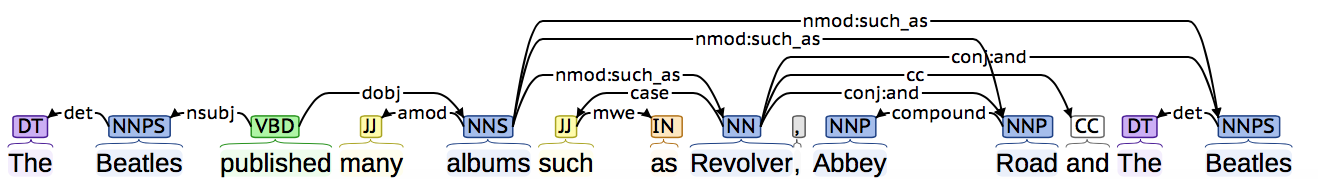
\includegraphics[width=7.7cm, height=1.2cm]{stanford}
	\caption{Esempio di una frase di tipo lista}
\end{figure}

Le frasi tra le entità sono state quindi passate ad un filtro per trovare quelle relazionali. Questa operazione snellisce di molto la quantità di triple estratte dalle frasi iniziali eliminando la maggior parte degli spezzoni di testo tra entità poiché il filtro è molto restrittivo, garantendo in output delle frasi che quasi sicuramente esprimono una relazione tra due entità.

\subsection{Etichettatura}
A questo punto, abbiamo considerato le entità di ogni tripla per verificarne l'effettiva presenza all'interno del grafo di DBpedia, sia in quello fidato che in quello non fidato.

Le triple cosiddette "etichettate" rappresentano fatti già presenti nel KG e sono utili per ricavare una mappatura tra le frasi che legano le entità e le relazioni ad esse accomunabili.

Quelle "non etichettate" sono invece candidate a rappresentare quella parte di conoscenza in più che il nostro lavoro tenta di estrarre, ampliando l'informazione della base di conoscenza.

Le frasi hanno subito una elaborazione molto leggera per pulire le frasi e ricondurre quelle più particolari a forme più generali in modo da non perdere informazione (e.g.: \textit{was born in} e \textit{was Born in} sono state assimilate alla stessa frase)

\subsection{Scoring}

Ogni frase è associata ad una o più relazioni definite da DBpedia, ma ovviamente queste corrispondenze potrebbero non rispettare l'effettiva semantica delle frasi stesse. (discuss da rivedere) Abbiamo quindi assegnato ad ogni frase un punteggio per definire l'appartenenza o meno ad una relazione considerando principalmente il numero di volte che esse sono associate con la relazione in esame. In questo modo abbiamo cercato di penalizzare frasi che esprimono concetti molto generici, ovvero che compaiono in molte relazioni, poiché non danno molta fiducia sulla correttezza dell'associazione.

Il punteggio viene assegnato tenendo conto del numero di volte che la frase è collegata alla determinata relazione ( $c(p,r_i)$ ), del conteggio totale delle sue occorrenze in tutte le relazioni ( $\sum_{j \in R} c(p,r_j)$ ) e del numero di relazioni a cui è associata ( $c(R|p)$ ) secondo la seguente formula: (discuss suddividere la formula con la parte centrale raccolta nella probabilità)
\[score(p,r_i)=c(p,r_i)\cdot\frac{c(p,r_i)}{\sum_{j \in R}c(p,r_j)}\cdot \frac{1}{c(R|p)} \]
In questo modo una frase otterrà un punteggio maggiore quanto più compare associata alla relazione in questione rispetto al numero totale di occorrenze, penalizzando inoltre le frasi in base al numero di relazioni a cui sono associate, poiché si tratta di forme con molta generalità e utilizzate per esprimere un grande insieme di relazioni diverse. Questo score può penalizzare (discuss ci sono frasi che non esistono, generalità di frasi tipo "is a")

\subsection{Estrazione dell'informazione}

Nella parte finale prendiamo le 20 frasi (o tutte se ce ne sono meno) con punteggio più alto per ogni relazione e le utilizziamo per estrarre fatti. (discuss gab descrive K) Ogni tripla inoltre per essere considerata valida, deve rispettare i vincoli che la relazione impone su DBpedia per soggetto e oggetto. Ad esempio, la frase "\textit{was born in}" è valida per la relazione \textit{birthPlace} se la prima entità è del tipo "Person" e la seconda del tipo "Place".

\section{VALUTAZIONE}

\end{document}